\chapter{Week 5: Data-analyse in Python}

We hebben inmiddels een gedegen bassis kennis van \textit{Python} opgedaan gedurende dit vak. We hebben o.a. geleerd over loops, lijsten, functies en IO aansturing in \textit{Python}, en de vershillen gezien met \textit{C}. Een van de concepten die nog onbelicht is gebleven is het zogeheten 'object georiënteerd programmeren' (of \textit{OOP}).
Omdat dit een van de belangrijkste en handigste concepten van het programmeren is van de afgelopen decenia, én omdat we stiekem er toch al flink mee gewerkt hebben, gaan we in dit hoofdstuk ook dit thema belichten. Daarnaast gaan we deze week aan de slag met \textit{packages}, handige software bibliotheken die de functionaliteit van onze \textit{Python} omgeving flink kunnen uitbreiden. 

\section{Object georiënteerd programmeren}\index{Object georiënteerd programmeren}
Zoals je wellicht al zou verwachten, focust het software design principe genaamd 'object georiënteerd programmeren' (OOP), zich vooral op 'objecten'. Objecten bestaan uit variabelen en functies. Waarbij je de variabelen kunt zien als eigenschappen van het object en functies als gedrag ervan. Lekker abstract hè? \\

Een voorbeeldje maakt het hopelijk wat duidelijker. Stel je voor: je wilt op een object georiënteerde manier naar een cirkel kijken. Allereerst ga je dan nadenken over welke eigenschappen jouw cirkel zou moeten hebben. Een cirkel heeft (in dit voorbeeld) maar één eigenschap: zijn straal. Dit wordt de variabele van ons cirkel-object, onthoud deze even. \\
\newpage
Daarnaast gaan we kijken naar het 'gedrag' van ons cirkel-object. Dat wil zeggen, we stellen ons de vraag, wat willen we allemaal met onze cirkel doen? Voor dit voorbeeld wil ik graag de oppervlakte en de omtrek van de cirkel makkelijk kunnen bepalen. Dit worden de twee functies van van ons object: 
\begin{figure}[h!]
\centering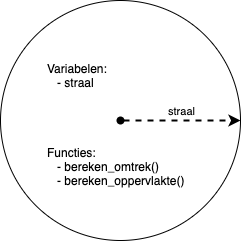
\includegraphics[scale=0.75]{Pictures/chapter07/cirkel.png}
\caption{Ons cirkel-object heeft een straal, en kan (op basis daarvan) de omtrek en oppervlakte van zichzelf berekenen.} 
\label{fig:cirkel} % Unique label used for referencing the figure in-text
%\addcontentsline{toc}{figure}{Figure \ref{fig:webserver}} % Uncomment to add the figure to the table of contents
\end{figure}

In code kunnen we dat nu op de volgende manier hiervan een blauwdruk van onze cirkel vastleggen:

\inputpython{code/chapter07/obj1.py}

We kunnen hier wel even kort doorheen lopen, om het concept wat hier gemaakt is goed te snappen. Allereerst wordt uit de \pyth{math} bibliotheek \pyth{pi} geïmporteerd, zodat we kunnen rekeken met $\pi$. Daarna wordt het interessant want op regel $4$ maken we een klasse-definitie van we onze cirkel, via het woordje \pyth{class}. Dit kun je zien als een soort blauwdruk van ons object, zodat we die later kunnen gebruiken. De naam van onze \pyth{class} is \pyth{Cirkel}, want klasse-definities schrijf je altijd met een hoofdletter. \\

Daarna is er op regel $5$ te zien dat we onze \pyth{Cirkel} een variabele \pyth{r} heeft, deze stelt de straal van de cirkel voor. En we hebben deze een standaard waarde $10$ gegeven. \\

Op regel $7$ en $12$ worden twee functies gedefinieerd, zoals als het goed is bekend voor moet komen. Het enige dat er een beetje gek aan is, is dat argument \pyth{self}. En dit is ook een bijzonder maar erg nuttig ding. Hiermee kan je namelijk de klasse-variabelen benaderen. Dus als je iets wil doen met de straal van de cirkel, gebruik je in de functies \pyth{self.r} (in plaats van enkel \pyth{r}). Je hoeft die \pyth{self} allleen te typen bij defineren van de klasse-functies. Bij het aanroepen wordt dit argument automatisch door \textit{Python} gevuld en hoef je deze dus ook niet mee te geven dan. \\

Laten we onze nieuwe klasse-definitie eens gebruiken. Sla het bovenstaande stukje code op als $cirkel.py$. Op deze manier kunnen we 'm nu importeren in een ander stukje code. Hieronder volgt een stukje code waarin onze \pyth{Cirkel} daadwerkelijk wordt gebruikt:

\inputpython{code/chapter07/obj1_use.py}

\begin{remark}
Let op: Importeren op deze manier werk alleen als beide bestanden in dezelfde folder staan.
\end{remark}

Ook dit stukje code heeft wellicht een beetje uitleg nodig. Op de eerste regel importeren we ons bestand \pyth{cirkel} en uit dat bestand willen we onze klasse-definitie \pyth{Cirkel} gebruiken. Je kunt dus meerdere klasse-definities in een bestand zetten en je importeert alleen diegene die je wilt gebruiken. \\ 

Op regel $4$ wordt (eindelijk) daadwerkelijk een object gemaakt van onze klasse-definitie. Het object heeft de naam \pyth{my_circle} en is dus van het type \pyth{Cirkel}. 

\begin{remark} 
Komt deze regel bekend voor? Toen ik eerder stelde dat we stiekem al vaker met object georiënteerd programmeren hebben gewerkt, is dit waar ik op doelde. \\
Zo hebben bijv. een tijdje terug al op deze manier een \pyth{LED} en een \pyth{Button} aangemaakt (\pyth{led = LED(17)} en \pyth{btn = Button(2)}). De klasse-definities van deze stonden namelijk in de package \pyth{gpiozero}. Zelf bij de \textit{Arduino} gebruikten we dit soms op plekken bijv. \pyth{Serial.print();}
\end{remark}

Na het aanmaken van het object \pyth{my_circ}, kunnen we deze gebruiken en bijv. de functies die het heeft aanroepen. Dit gebeurt op regel $7 \& 8$ (zie je dat hier niets meer te zien is van de \pyth{self}). De waardes die de functies teruggeven worden opgeslagen in de variabelen \pyth{omt} en \pyth{opp} en deze worden uiteindelijk in de laatste $3$ regels op een nette manier naar het scherm geschreven: \\ 

\begin{python}
Deze cirkel heeft een straal van: 10cm.
En daarmee een omtrek van: 62.83cm.
En heeft een oppervlakte van: 314.16cm^2.
\end{python}

\newpage

\subsection{Constructors}\index{Constructors}
Het voordeel van object geörienteerd programmeren is dat de gemaakte objecten makkelijk herbruikbaar (en uitbreidbaar) zijn. Hierdoor is je code ook makkelijker te onderhouden en is er als het goed is een duidelijke structuur in je projecten terug te zien. \\

In ons \pyth{Cirkel}-voorbeeldje is de herbruikbaarheid van de code nog niet zo duidelijk, omdat de cirkel in dit geval alijd een straal van $10$cm heeft. Je zou deze eigenlijk flexibel willen aanpassen naar je wensen. Dit kan heel mooi met een \textit{constructor}. De \textit{constructor} is de functie die wordt aangeroepen door \textit{Python} (dus automatisch) wanneer je een object aanmaakt, dus in dit geval dus bij de regel: \pyth{my_circle =} \pyth{Cirkel()}. \\ 

Zo'n \textit{constructor} is dus optioneel, we hebben 'm immers nog niet aangemaakt. Laten we er nu eentje maken voor onze cirkel-definitie. Een constructor is gewoon een functie, maar met een vaste (en wat gekke) naam: \pyth{__init__(self)} (met $2$ keer $2$ liggende streepjes). Zie het onderstaande voorbeeld:

\inputpython{code/chapter07/obj2.py}

In de bovenstaande code is niet veel veranderd ten opzichte van de vorige versie van \textit{cirkel.py}. De klasse-variabele \pyth{r} is nu standaard $0$ en dient nu een waarde te krijgen via de constructor. Ook zijn de functies wat compacter geschreven, maar functioneel exact hetzelfde. \\

De daadwerkelijke constructor zien we op regels $7$-$9$. Zoals gezegd heeft deze een vaste naam, en naast het argument \pyth{self} is er ook een argument \pyth{r}. Hiermee kun je dus de gewenste straal opgeven als je een object maakt. Laten we dat eens doen:

\begin{python}
from cirkel import Cirkel

# Maak een Cirkel, met de naam my_circ en een straal van 5:
my_circ  = Cirkel(5)   

# Maak een Cirkel, met de naam my_circ2 en een straal van 25:
my_circ2 = Cirkel(25) 
\end{python}

Bij het aanmaken van het objet, bepalen we dus pas de straal van de cirkel. En hebben we op deze manier een flexibel object gemaakt die we steeds opnieuw kunnen gebruiken en makkelijk kunnen uitbreiden. Willen we bijv. een functie wijzigen of toevoegen, dan hoeven we dat maar op een plek te doen: in de klasse-definitie in \pyth{cirkel.py}. Overal waar we dan een object ervan gebruiken zal deze nieuwe functionalteit dan beschikbaar komen. 

\newpage

Object georiënteerd programmeren is niet het makkelijkste onderwerp om compleet te begrijpen. Als je hier voor het eerst naar kijkt kan dit wellicht nog een beetje criptisch en abstract overkomen. Daarom geef ik in dit hoofdstuk nog een voorbeeld voordat we verder gaan met andere onderwerpen. \\

Laten we het eens proberen met wat simpele hardware, een LED. We gebruikten vaak de \pyth{LED} klasse uit de \pyth{gpiozero} package. Stel nu dat die package niet bestond en we het enkel moesten doen met de 'klassieke' \pyth{RPi.GPIO} package. Dan zouden we met de kennis die we inmiddels over OOP hebben opgedaan, zelf een LED-klasse maken. \\

Hierbij dienen we weer eerst af te vragen, wat zijn de eigenschappen en functies van een led. Een led zit altijd aangesloten aan een bepaalde pin en heeft daarnaast een status ('aan' dan wel 'uit'). Qua functionaliteit wil je een led aan kunnen zetten, uit kunnen zetten, en eventueel ook willen schakelen (togglen, uitzetten als hij aan is, en vice versa): 

\begin{figure}[h!]
\centering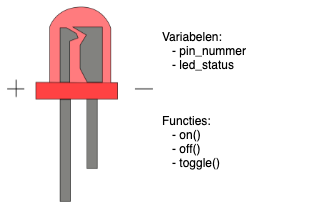
\includegraphics[scale=0.5]{Pictures/chapter07/led.png}
\caption{Led-object met 'pin\_nummer' en een 'status' en kan aan, uit of geschakeld worden.}
\label{fig:led} % Unique label used for referencing the figure in-text
\end{figure}

Als we ons herinneren uit vorige weken, kunnen we met \textit{RPi.GPIO} al deze functionaliteiten uitwerken. We gaan nu deze package gebruiken om een object georiënteerde \pyth{Led}-klasse te maken (die functioneel dus vergelijkbaar is met de \pyth{LED}-klasse uit \textit{gpiozero}). Sla dit op als \pyth{my_led.py}.

\inputpython{code/chapter07/led.py}

In de code hierboven gebruiken we dus de package \textit{RPi.GPIO} om een OOP versie van een Led te maken. Op regel $1$ importeren we deze package. De twee variabelen van de Led, \pyth{led_pin} en \pyth{status} zijn te vinden onder de klasse-definitie. \\
In de constructor gebeurt alle setup code. De klasse-variablen krijgen hun waarde (regel $12$ en $13$). Daarna wordt de poort geïnitieerd als uitgang. En uieindelijk wordt voor de netheid, de huidige status geschreven naar de led pin. Als status nu \pyth{True} is, gaat de Led aan. Is deze \pyth{False}, blijft hij uit.
\begin{remark}
Valt je op dat in constructor de \pyth{default_state} al een waarde krijgt? (\pyth{False}). Dit is een standaard waarde. Zodat bij het aanmaken van daadwerkelijke object, je het argument \pyth{default_state} niet per se mee hoeft te geven. Oftewel, je kunt ons Led-object op deze manieren aanmaken:
\begin{python}
from my_led import Led

voorbeeld_led = Led(17, False)  # Led op pin 17, standaard uit  
voorbeeld_led = Led(17)         # Led op pin 17, standaard uit  
voorbeeld_led = Led(17, True)   # Led op pin 17, standaard aan  
\end{python}
\end{remark}
Daarna volgen de functies van de led. Deze zullen er als het goed is niet verrassend uitzien. \pyth{on()} en \pyth{off()} zetten de led respectievelijk aan en uit. En de \pyth{toggle()} functie zet de led uit, als deze aan was, en aan als deze uit was. Ook wordt overal de nieuwe status van de led opgeslagen. \\

De klasse-definitie is dan als het volgt bijv. te gebruiken:
\begin{python}
from my_led import Led
from time import sleep

mijn_led = Led(17)  # Led op pin 17

while True:
  mijn_led.on()
  sleep(1)
  mijn_led.off()
  sleep(1)
\end{python}

\begin{exercise}
Zie jij verschillen met de code op blz. \pageref{sec:piledobj}?
\end{exercise}

\newpage

\section{Packages}\index{Packages}
Een \textit{Package} in \textit{Python} is een verzameling van modules. Deze modules kunnen we weer in onze code gebruiken door deze te importeren met \pyth{import}. We hbben er in middel al een aantal van gebruikt bijv.: \pyth{math, time, gpiozero, RPi}, maar deze worden allemaal al standaard meegeleverd op bijv. de \textit{Raspberry Pi}. Je kunt ze ook heel eenvoudig zelf toevoegen aan je \textit{Python} omgeving, door gebruik te maken van \pyth{pip}. Dit programma kun je aanroepen vanaf de terminal:

\begin{lstlisting}[language=bash]
python3 -m pip install <naam_package>
\end{lstlisting}

\begin{remark}
Je hebt ongetwijfeld al een hele lijst geïnstalleerd zonder dat je het wist, je kunt het bekijken door het onderstaande in een terminal in te typen: 
\begin{lstlisting}[language=bash]
python3 -m pip list
\end{lstlisting}
En als je wat schijfruimte wilt vrij maken door packages te verwijderen die je niet langer gebruikt, kan dat met:
\begin{lstlisting}[language=bash]
python3 -m pip uninstall <naam_package>
\end{lstlisting}
\end{remark}

Om een beetje bekend te raken met \textit{pip}, gaan we als voorbeeld een kleine package installeren genaamd \pyth{camelcase}:
\begin{lstlisting}[language=bash]
python3 -m pip install camelcase
\end{lstlisting}

Probeer nu het volgende scriptje te draaien:
\begin{python}
from camelcase import CamelCase     # importeer onze nieuwe aanwinst

c = CamelCase()                     # Nodig om de package te kunnen gebruiken.
txt = 'pip onder de knie krijgen!'  # De tekst die omgezet dient te woren.

print(c.hump(txt))                  # Pas camelcase toe op de tekst.
\end{python}
Als dat lukt, is de module juist geïnstalleerd en heb je de basis van \textit{pip} onder de knie! (Deze packages worden overigens gedownload vanaf \url{https://pypi.org/}, kijk er gerust eens na en wellicht kom je er interressante tegen tussen de bijna 350.000 packages.) \\
Het aanpassen van hoofdletters is echter niet al te spannend, dus gaan we verder met een package waar we echt iets aan hebben: \textit{matplotlib}. 

\newpage
\section{matplotlib}\index{matplotlib}

\begin{figure}[h!]
\centering
\includegraphics[scale=0.25]{Pictures/chapter07/matplotlib_logo.png}
% \caption{\small \textit{Matplotlib} logo. Bron: \url{https://matplotlib.org}}
\label{fig:mpllogo} % Unique label used for referencing the figure in-text
%\addcontentsline{toc}{figure}{Figure \ref{fig:webserver}} % Uncomment to add the figure to the table of contents
\end{figure}

Matplotlib is een verzameling aan tools voor het maken en bewerken van grafieken. 
\begin{exercise}
  Installeer Matplotlib
\end{exercise}

Om het te gebruiken in z'n meest simpele vorm zorg je ervoor dat je een reeks $x$-waardes hebt, en een reeks bijbehorende $y$-waardes. Deze kun je dan plotten (het doorrekenen van alle data van de grafiek) en de resulterende grafiek kun je tonen op het scherm:

\inputpython{code/chapter07/plot1.py}

Hieruit rolt grafiek \ref{fig:plot1} uit:
\begin{figure}[h!]
\centering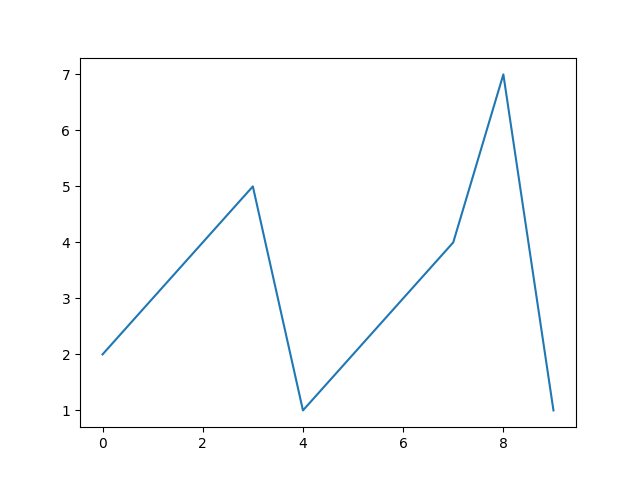
\includegraphics[scale=0.7]{Pictures/chapter07/plot1.png}
\caption{Simpele plot met \textit{Matplotlib}}
\label{fig:plot1} % Unique label used for referencing the figure in-text
%\addcontentsline{toc}{figure}{Figure \ref{fig:webserver}} % Uncomment to add the figure to the table of contents
\end{figure}

\newpage

\begin{remark}
Kreeg je bij het runnen van bovenstaande code op de \textit{Pi} een error, in de trant van \textit{'Error retrieving accessibility bus address'}? Dan kan het zijn dat je een module in Linux mist, open een terminal en voer in: 
\begin{lstlisting}[language=bash]
sudo apt update
sudo apt install at-spi2-core
\end{lstlisting}
\end{remark}

Een grafiek is natuurlijk pas echt bruikbaar als deze netjes is opgemaakt met duidelijke labels voor de assen en eventueel een titel en een legenda. Ook dat is snel gepiept met \textit{matplotlib}. In het onderstaande stuk code voegen we dit toe aan ons eerdere script. Daarnaast is er een extra set met $y$-waardes toegevoegd, om $2$ verschillende meetmomenten na te bootsen.

\inputpython{code/chapter07/plot2.py}

De bonenstaande code produceert onderstaande grafiek \ref{fig:plot2}:
\begin{figure}[h!]
\centering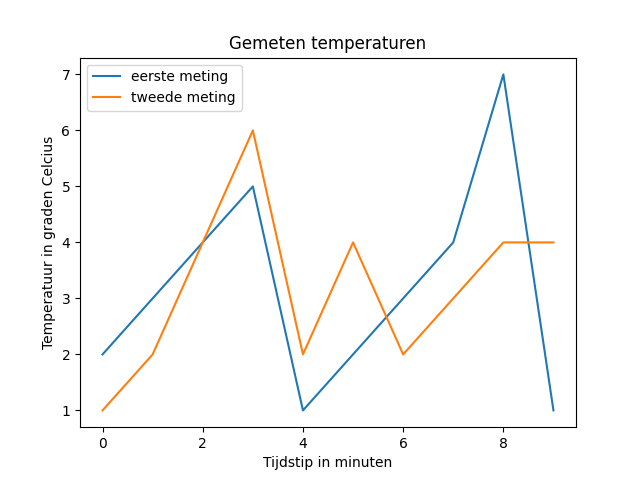
\includegraphics[scale=0.7]{Pictures/chapter07/plot2.png}
\caption{Uitgebreidere plot met \textit{Matplotlib}}
\label{fig:plot2} 
%\addcontentsline{toc}{figure}{Figure \ref{fig:webserver}} % Uncomment to add the figure to the table of contents
\end{figure}

\begin{exercise}
Zorg dat de eerste lijn rood gekleurd (\pyth{color}) wordt, en de tweede lijn groen en gestippeld (\pyth{linestyle}). \\
\textbf{TIP: } Gebruik hiervoor de documentatie van de packge op: \url{https://matplotlib.org}. 
\end{exercise}

\newpage

\subsection{NumPy}\index{NumPy}

\begin{figure}[h!]
\centering
\includegraphics[scale=0.5]{Pictures/chapter07/numpy_logo.png}
% \caption{\small \textit{Matplotlib} logo. Bron: \url{https://matplotlib.org}}
\label{fig:numpylogo} % Unique label used for referencing the figure in-text
%\addcontentsline{toc}{figure}{Figure \ref{fig:webserver}} % Uncomment to add the figure to the table of contents
\end{figure}

De mogelijkheden van \textit{matplotlib} kunnen enorm uitgebreid worden in combinatie met andere packages. Een voor de hand liggende keuze daarin is bijvoorbeeld \textit{NumPy}. Die een enorm scala aan wiskundige tools met zich meebrengt. 

\begin{exercise}
Installeer NumPy 
\end{exercise}
We kunnen met de combinatie \textit{NumPy} en \textit{matplotlib} bijv. elke wiskunde functie die we kunnen bedenken op een makkelijke en overzichtelijke wijze plotten. Superhandig voor je wiskunde huiswerk ;). Als voorbeeldje volgt hieronder een klein scriptje die $y = sin(x)$ plot op een bereik van $-\pi$ tot $\pi$:

\newpage

\inputpython{code/chapter07/plot_numpy.py}

De bonenstaande code produceert onderstaande grafiek \ref{fig:plot3}:
\begin{figure}[h!]
\centering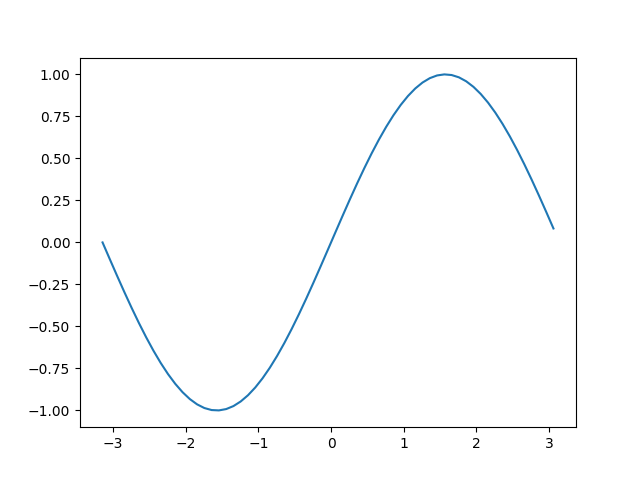
\includegraphics[scale=0.7]{Pictures/chapter07/sin.png}
\caption{Een sinus-functie tekenen met \textit{Matplotlib} en \textit{NumPy}.}
\label{fig:plot3} 
%\addcontentsline{toc}{figure}{Figure \ref{fig:webserver}} % Uncomment to add the figure to the table of contents
\end{figure}

Op regel $5$ wordt hier een reeks aan getallen gegenereerd door de \pyth{np.arange()}-functie. Valt je op dat deze functie nagenoeg hetzelfde eruit ziet (en werkt!) als de ingebouwde \pyth{range()}-functie? Het verschil zit 'm in dat \pyth{np.arange()} ook reeksen met komma-getallen (floats) kan genereren. \\ 
Om een soortgelijke reden gebruiken we op regel $7$ \pyth{np.sin()} in plaats van \pyth{math.sin()}. De sinus functie uit \textit{NumPy} kan namelijk de sinus van een hele reeks getallen uitrekenen en dit weer teruggeven als een reeks getallen. De sinus-functie uit \pyth{math} kan enkel de sinus uitrekenen op $1$ getal per keer.
 
% \subsection{pip}\index{pip}
\newpage

\section{Pandas}\index{Pandas}
\begin{figure}[h!]
\centering
\includegraphics[scale=0.2]{Pictures/chapter07/pandas_logo.png}
% \caption{\small \textit{Matplotlib} logo. Bron: \url{https://matplotlib.org}}
\label{fig:pandaslogo} % Unique label used for referencing the figure in-text
%\addcontentsline{toc}{figure}{Figure \ref{fig:webserver}} % Uncomment to add the figure to the table of contents
\end{figure}

% \subsection{Excel file edit}\index{Excel file edit}
Het tekenen van grafieken wordt een stuk intteressanter als je veel input data hebt. Die kun je bijvoorbeeld krijgen door een sensor periodiek te meten, maar ook door een spreadsheet in te laden. De package \textit{pandas} gaat je bij dat laatste flink helpen.

\begin{exercise}
Installeer de package \textit{Pandas} en z'n verschillende parsers:
\begin{lstlisting}[language=bash]
python3 -m pip install pandas odfpy openpyxl xlrd
\end{lstlisting}
De laatste drie packages die hier worden geïnstalleerd zijn resp. nodig voor support van $.ods$- (LibreOffice), $.xslx$- (Microsoft Excel) en $.xls$- (Oude Microsoft Excel) bestanden. Mocht je bepaalde bestandsformaten niet gaan gebruiken, kun je die uiteraard overslaan.
\end{exercise}

Naast de \textit{Python} packages ben je natuurlijk ook een programma nodig dat spreadsheets kan maken en bewerken. Op je laptop gebruik je hier ongetwijfeld Microsoft Excel voor. Voor de Raspberry Pi moet je hier waarschijnlijk nog even een programma voor installeren. Voor een complete office suite variant, kun je bijv. LibreOffice installeren. Dit is een gratis, en een heel complete vervanger voor Microsoft Office (die overigens ook prima draait op je laptop ;) ).\\\\ 
Heb je nu geen zin in een grote download, kun je ook kiezen voor Gnumeric. Dat is gewoon een basic spreadsheet editor zonder poespas, maar wel met alle functionaliteit in huis die we tijdens dit vak nodig zijn.

\begin{exercise}
Installeer op basis van je voorkeur één spreadsheet programma op je Pi:
\begin{lstlisting}[language=bash]
sudo apt install libreoffce
sudo apt install gnumeric
\end{lstlisting}
\end{exercise}

Als voorbeeld heb ik de volgende spreadsheet aangemaakt: Een tabel met twee kolommen: 'Tijdstip' en 'Waarde', met elk $50$ rijen/waardes: 
\begin{figure}[h!]
\centering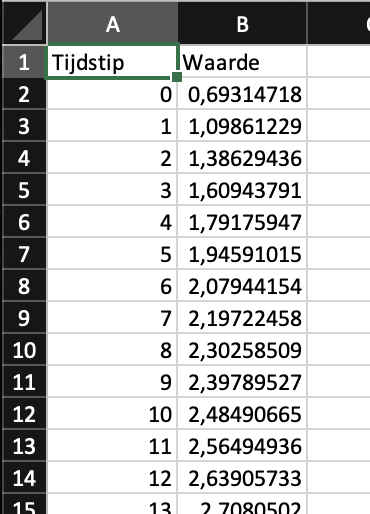
\includegraphics[scale=0.5]{Pictures/chapter07/excel1.png}
\caption{Voorbeeld spreadsheet gemaakt in Excel.}
\label{fig:excel1} % Unique label used for referencing the figure in-text
%\addcontentsline{toc}{figure}{Figure \ref{fig:webserver}} % Uncomment to add the figure to the table of contents
\end{figure}

\newpage

Deze spreedsheet is dan met \textit{pandas} als volgt heel eenvoudig in te laden:
\inputpython{code/chapter07/exc1.py}

\begin{remark}
Heb je nu een spreadsheet met meerdere tabladen gemaakt en wil je een specifiek blad inladen met de naam 'Blad1'? Dat kan prima. Pas dan regel $4$ aan van de code naar: \\
\pyth{df = pd.read_excel('excel1.xlsx', sheet_name='Blad1')}
\end{remark}

Dit stukje code leest de $.xlsx$-bestand in, en print daarna alle namen van de kolommen op het scherm:
\begin{python}
Tijdstip
Waardes
\end{python}

Deze namen kunnen we daarna gebruiken om de daadwerkelijke data te benaderen en bijvoorbeeld te printen met \textit{matplotlib}:

\inputpython{code/chapter07/exc2.py}

Dit bovenstaande stukje code levert uiteindelijk de volgende grafiek op:

\begin{figure}[h!]
\centering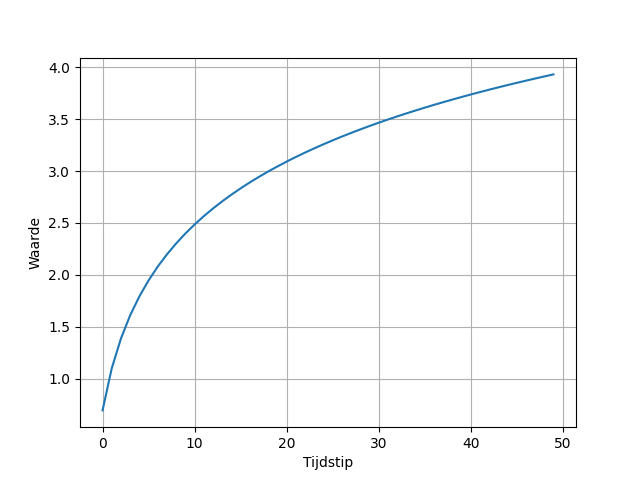
\includegraphics[scale=0.7]{Pictures/chapter07/plot3.png}
\caption{Plot gemaakt vanuit spreadsheet.}
\label{fig:plot3} % Unique label used for referencing the figure in-text
%\addcontentsline{toc}{figure}{Figure \ref{fig:webserver}} % Uncomment to add the figure to the table of contents
\end{figure}

\begin{remark}
Nerdy tip: Je kunt ook in plaats van zelf de x- en y-labels een naam te geven, dit af laten hangen van de gevonden kolomnamen:
\begin{python}
plt.xlabel(df.columns[0])
plt.ylabel(df.columns[1])
\end{python}
\end{remark}

\newpage

Andersom kan natuurlijk ook: Je hebt data in je \textit{Python} script, en dat wil je opslaan als een spreadsheet. Dat is wat we met het volgende stukje code doen:

\inputpython{code/chapter07/toexc.py}

Het gegenereerde bestand kunnen we openen met ons spreadsheet-programma, en zal er dan zo uitzien:

\begin{figure}[h!]
\centering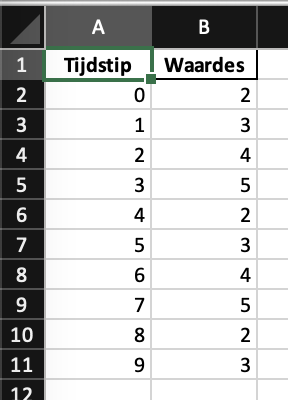
\includegraphics[scale=0.7]{Pictures/chapter07/excel2.png}
\caption{Spreadsheet gegenereerd vanuit \textit{Python}}
\label{fig:excel1} % Unique label used for referencing the figure in-text
%\addcontentsline{toc}{figure}{Figure \ref{fig:webserver}} % Uncomment to add the figure to the table of contents
\end{figure}

\newpage

\section{Huiswerkopdrachten}\index{Huiswerkopdrachten}
\begin{exercise}
Maak een klasse \textit{Persoon} aan. Geef 'm als variabelen een \textit{naam}, \textit{leeftijd} en een \textit{geslacht}. Geef hem een functie \pyth{zeg_hoi()}, waarmee hij/zij zichzelf kan voorstellen (met een \pyth{print()}-statement). 
\end{exercise}

\begin{exercise}
Maak op basis van de Led-voorbeeldklasse een klasse aan voor een RGB led (een drie kleuren-led). Doe dit op basis van \textit{RPi.GPIO} met $3$ verschillende leds (een voor elke kleur). Geef de RGB naast een constructor, een aantal fucties: bijv. \pyth{rood()}, \pyth{groen()}, \pyth{blauw()}, \pyth{uit()} en bedenk zelf ook nog kleur-combinaties a.h.v. de $3$ leds.
\end{exercise}

\begin{exercise}
Op regel $8$ van het de laatste voorbeeld code gebruiken we de \pyth{zip()}-functie. Ga na in wat deze functie precies doet met 2 lijsten. 
\end{exercise}

\begin{exercise}
Plot (in $1$ grafiek) met \textit{matplotlib} en \textit{NumPy} de functies: \\
$y_{1}=\sin(2\cdot x)$ en $y_{2}=4\cdot\cos(4\cdot x)$ tussen $-2\pi$ en $2\pi$. Zorg ook voor een duidelijke legenda.
\end{exercise}

\begin{exercise}
\label{exc7:exc2}
Vraag van de gebruiker steeds een nummer, net zolang tot deze 'klaar' intypt. \\
Voeg alle getallen die de gebruiker intypte steeds toe aan een lijst en print hier (als de gebruiker klaar is) een nette grafiek van. (Begin voor de x-waardes te tellen bij $0$, en tel er steeds 1 bij op, voor elk ingevoerd getal).
\end{exercise}

\begin{exercise}
\label{exc7:exc3}
Breid het het programma van opdracht \ref{exc7:exc2} uit, zodat het programma ook een Excel sheet opslaat met alle ingevoerde cijfers.
\end{exercise}

\begin{exercise}
Maak een eigen klasse \textit{Xlsx\_writer} met de volgende variabelen: 
\begin{itemize}
  \item[-]{\makebox[2cm] {filename\hfill}   $\rightarrow$ Een bestandnaam (bijv. "file.xlsx").}
  \item[-]{\makebox[2cm] {x\_waardes\hfill} $\rightarrow$ Een lijst met x-waardes.}
  \item[-]{\makebox[2cm] {y\_waardes\hfill} $\rightarrow$ Een lijst met y-waardes.}
  \item[-]{\makebox[2cm] {x\_label\hfill}   $\rightarrow$ (Optioneel) Een string met een label voor de x-waardes.}
  \item[-]{\makebox[2cm] {y\_label\hfill}   $\rightarrow$ (Optioneel) Een string met een label voor de y-waardes.}
\end{itemize}

Geef 'm een functie: \pyth{sla_op()}, waarmee je alle data verwerkt en het bestand opslaat als een excel-sheet. Verwerk deze klasse in je programma van \ref{exc7:exc3}.
\end{exercise}


